\documentclass[10.7pt, onecolumn]{article}

\usepackage[letterpaper, margin=2.54cm, top=2.54cm]{geometry}
\usepackage[super,comma,sort&compress]{natbib}
\usepackage{lmodern}
\usepackage{authblk} % To add affiliations to authors
\usepackage{amssymb,amsmath}
\usepackage{wrapfig}
\usepackage{graphicx,grffile}
\usepackage[labelfont=bf,labelsep=period]{caption}
\usepackage{ifxetex,ifluatex}
\usepackage{fixltx2e} % provides \textsubscript
\usepackage{graphicx}
\usepackage{pdfpages}
\ifnum 0\ifxetex 1\fi\ifluatex 1\fi=0 % if pdftex
  \usepackage[T1]{fontenc}
  \usepackage[utf8]{inputenc}
\else % if luatex or xelatex
  \ifxetex
    \usepackage{mathspec}
  \else
    \usepackage{fontspec}
  \fi
  \defaultfontfeatures{Ligatures=TeX,Scale=MatchLowercase}
    \setmainfont[]{Times New Roman}
    \setsansfont[]{Century Gothic}
    \setmonofont[Mapping=tex-ansi]{Consolas}
\fi
% use upquote if available, for straight quotes in verbatim environments
\IfFileExists{upquote.sty}{\usepackage{upquote}}{}
% use microtype if available
\IfFileExists{microtype.sty}{%
	\usepackage{microtype}
	\UseMicrotypeSet[protrusion]{basicmath} % disable protrusion for tt fonts
}{}

\usepackage{float}
\usepackage{lipsum}
\newtheorem{exm}{Example}


%==============================
% Customization to make the output PDF 
% look similar to the MS Word version
%==============================
% To prevent hyphenation
\hyphenpenalty=10000
\exhyphenpenalty=10000

% To set the sections font size
\usepackage{sectsty}
\allsectionsfont{\fontsize{10}{10}\selectfont}
%\sectionfont{\fontsize{10}{10}\selectfont}
\subsectionfont{\itshape\bfseries\fontsize{10}{10}\selectfont}
\subsubsectionfont{\normalfont\itshape}

% No new line after subsubsection
\makeatletter
\renewcommand\subsubsection{\@startsection{subsubsection}{3}{\z@}%
	{-3.25ex\@plus -1ex \@minus -.2ex}%
    {-1.5ex \@plus -.2ex}% Formerly 1.5ex \@plus .2ex
    {\normalfont\itshape}}
\makeatother

\makeatletter % Reference list option change
\renewcommand\@biblabel[1]{#1.} % from [1] to 1
\makeatother %

% To set the doc title font
\usepackage{etoolbox}
\makeatletter
\patchcmd{\@maketitle}{\LARGE}{\bfseries\fontsize{15}{16}\selectfont}{}{}
\makeatother

% No page numbering
\pagenumbering{gobble}

\makeatletter
\def\maxwidth{\ifdim\Gin@nat@width>\linewidth\linewidth\else\Gin@nat@width\fi}
\def\maxheight{\ifdim\Gin@nat@height>\textheight\textheight\else\Gin@nat@height\fi}
\makeatother

% Scale images if necessary, so that they will not overflow the page
% margins by default, and it is still possible to overwrite the defaults
% using explicit options in \includegraphics[width, height, ...]{}
\setkeys{Gin}{width=\maxwidth,height=\maxheight,keepaspectratio}
\setlength{\parindent}{0pt}
\setlength{\parskip}{6pt plus 2pt minus 1pt}
\setlength{\emergencystretch}{3em}  % prevent overfull lines
\providecommand{\tightlist}{%
  \setlength{\itemsep}{0pt}\setlength{\parskip}{0pt}}
\setcounter{secnumdepth}{0}
% Redefines (sub)paragraphs to behave more like sections
\ifx\paragraph\undefined\else
\let\oldparagraph\paragraph
\renewcommand{\paragraph}[1]{\oldparagraph{#1}\mbox{}}
\fi
\ifx\subparagraph\undefined\else
\let\oldsubparagraph\subparagraph
\renewcommand{\subparagraph}[1]{\oldsubparagraph{#1}\mbox{}}
\fi
%==============================
\usepackage{hyperref}
\hypersetup{
	unicode=true,
	pdftitle={NLP4Heatlh_Assignment3_Halim},
	pdfauthor={Jule Valendo Halim - 1425567},
	pdfkeywords={keyword1, keyword2},
	pdfborder={0 0 0},
	breaklinks=true
}
\urlstyle{same}  % don't use monospace font for urls
%==============================

% reduce space between title and begining of page
\title{\vspace{-2em} Investigating the Use of Statistical Tests in Machine Learning Models}
\author[ ]{\bf\fontsize{13}{14}\selectfont Jule Valendo Halim -1425567\vspace{-.7em}}
\affil[ ]{\bf\fontsize{13}{14}\selectfont University of Melbourne}
\date{} % add no date (by default date is added)

%==============================
\begin{document}
\maketitle
\vspace{-4em} %separation between the affiliations and abstract
%==============================

%==============================
\section{Abstract}\label{abstract}
%==============================
\subsection{Objective}

To investigate possible roles of statistical tests on natural language processing tasks through models for multi-label and multi-class classifiers.
\subsection{Materials}

Dataset containing online patient reviews of prescribed medication, provided by Zoolnori et al\cite{psyTAR1} and Zoolnori et al\cite{psyTar2}. The dataset contains annotated labels for each review sentence, along with the medication being reviewed.
\subsection{Methods}

Multi-label classification was performed with two different textual features, and each feature was trained on a logistic regression and transformer model. This resulted in 4 models. 

Multi-class classification was performed with three different textual features, and each feature was also trained on logistic regression and transformer models, resulting in 6 models.

Model prediction were then evaluated using traditional machine learning metrics such as accuracy, before then being evaluated using statistical tests.

\subsection{Results}

When comparing traditional machine learning metrics, transformer models generally outperform their logistic regression, except for one task-feature pair. Statistical test results were reported and interpretations were provided.
\subsection{Discussion}

Statistical result interpretations were discussed as possible model behaviours that could be further investigated. The difficulty of applying statistical tests on natural language processing tasks were also discussed.

\subsection{Conclusion}

Statistical tests provide valuable insight into model behaviour outside of traditional machine learning metrics. However, additional work is needed in creating a pipeline to investigate causes of possible model behaviour, as well as integration of assumption testing.

%==============================
\section{Introduction}\label{introduction}
%==============================
Statistical tests are a popular and long-standing method in multiple fields of science. However, studies in natural language processing (NLP) and machine learning (ML) do not generally include statistcal testing as part of their model evaluation. A survey on 233 published papers in the field of NLP showed that 132 of these papers did not report statistical significance\cite{statsPaper}. However, more studies have begun advocating for the use of these tests to show that experimental results are not coincidental\cite{statsPaper} and argue that a combination of NLP and statistical tests can provide a framework for the development of robust, high-throughput health NLP systems\cite{10.1197/jamia.M3028}. 

In this report, I aim to investigate the use of statistical tests on ML models that predict multi-label and multi-class  classification tasks using the statistical test workflow suggested by Rainio, Tauho, and Klén\cite{statsBased}, as seen in figure \ref{fig:statistical test workflow}. However, instead of comparing results from different test sets, this report compares different model feature inputs.

\begin{figure}[H]
  \centering
  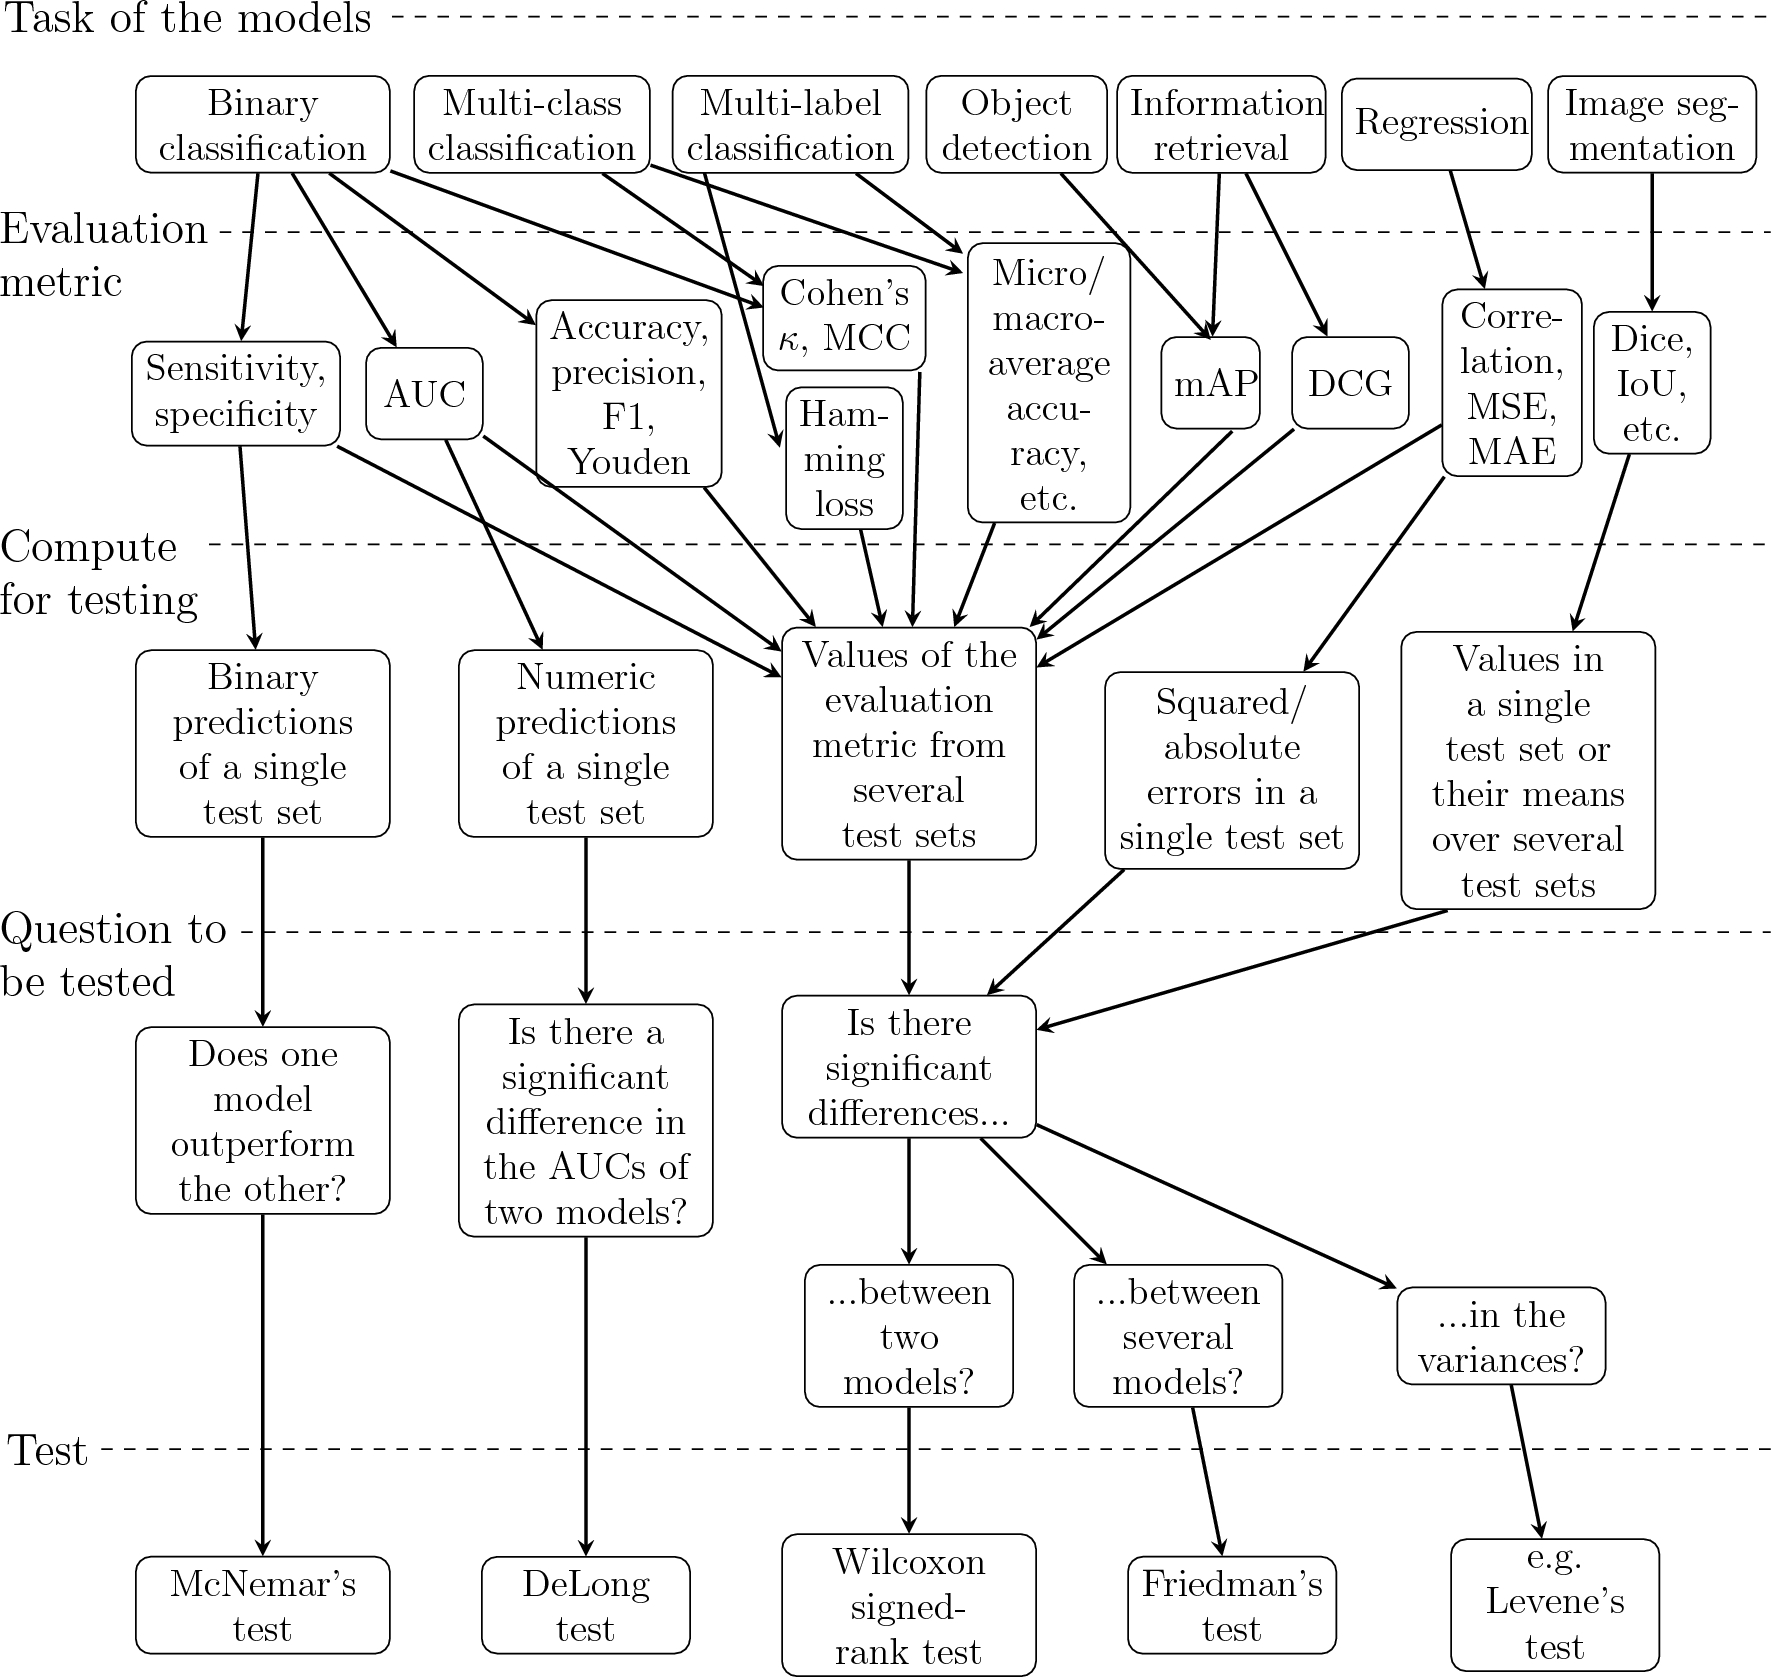
\includegraphics[width=\textwidth]{images/41598_2024_56706_Fig3_HTML.png}
  \caption{Statistical Workflow Provided by Rainio, Tauho, and Klén\cite{statsBased}}
  \label{fig:statistical test workflow}
\end{figure}
 
The Sentence\_Labeling sheet of the PsyTAR dataset used in this study is provided by Zoolnoori et al\cite{psyTAR1} and Zoolnori et al\cite{psyTar2}. This sheet contains three sections of interest. The first is sentences from online patient reviews of certain drugs. The second is annotations of certain labels, described below in table \ref{tab:6Labels}. The third is drug labels, which indicates which drug each sentence is reviewing.

Two classification tasks were performed using a baseline logistic regression model and a transformer model. The multi label class predicts six binary annotations, while the multi-class predicts four different drugs. For each model, different features will be used as inputs. The resulting predictions will be used for statistical tests in order to determine their statistical signifance. Specific details are described in the methods section.

%==============================
\section{Methods}\label{methods}
%==============================
% ASK ON WHETHER I NEED TO DESCRIBE IN DETAIL THE STATISTCAL TESTS USED

\subsection{Ethics Statement}

This study has one important ethical consideration, which is that 


\subsection{Preprocessing}
Two main preprocessing steps were done. Firstly, as the drug labels in the data were concatenated with review ID, the review ID was stripped and only the drug label was added to a new column. Secondly, the review text was preprocessed through tokenization, as well as stopword and punctuation removal. The dataset consists of 6009 records. The data was split into train, validation, and test sets using a 45:45:10 ratio.
\subsection{Multi-Label Classification}
Multi-label classification involves predicting six labels, as shown in table \ref{tab:6Labels}. Each label is a binary task (1 for present and 0 for absent), which has been manually annotated. This task aims to predict annotations for a given review text.

\begin{table}[H]
  \centering
  \begin{tabular}{|p{4cm}|p{3cm}|}
    \hline
    \textbf{Predicted Class} & \textbf{Description} \\
    \hline
    Adverse Drug Reactions (ADR) & - \\
    \hline
    Withdrawal Symptom (WD) & - \\
    \hline
    Effective (EF) & - \\
    \hline
    Ineffective (INF) & - \\
    \hline
    Sign/Symptom/Illness (SSI) & Text contains explicit SSI as a result of the drug \\
    \hline
    Drug Indication (DI) & Text contains SSI that is currently being addressed by the drug \\
    \hline
  \end{tabular}
  \caption{The six labels predicted by multi-label classifiers}
  \label{tab:6Labels}
\end{table}

\subsubsection{Selected Features}

Two features were used for multi-label classification. The first is the preprocessed sentences without any additional features. From here on, references to this task-feature pair will be referred as Task 1 Feature 1. The second contains the drug name added to the start of the review text. This will be referred to as Task 1 Feature 2.

\subsubsection{Logistic Regression}
The logistic regression model performed Term Frequency Inverse Document Frequency (TF-IDF) vectorization on the input text. A multi-output classifier was built upon a logistic regression model, which was then tuned using hyperparameter tuning.

\subsubsection{Transformer}
The transformer model uses a pre-trained BERT model, which was trained on a downstream task in order to create a multi-label transformer classifier. Binary cross-entropy loss (BCE) with logits (a sigmoid layer) loss was used for loss calculation. BCE is well-suited for binary classification\cite{xu2023learning} such as this task, and using the logits replaces negative values with 0s to avoid large negative numbers. Table \ref{tab:task1Parameters} shows the configurations used in the transformer. 15 epochs were done for each transformer model, resulting in convergence of loss and accuracy. The training and validation loss and accuracies are shown in appendix B.

\begin{table}[H]
  \centering
  \begin{tabular}{|p{4cm}|p{4cm}|}
    \hline
    \textbf{Parameter} & \textbf{Value} \\
    \hline
    hidden\_size & 768 \\
    \hline
    num\_hidden\_layers & 24 \\
    \hline
    num\_attention\_heads & 12 \\
    \hline
    intermediate\_size & 3072 \\
    \hline
    num\_labels & 6 \\
    \hline
    optimizer & AdamW \\
    \hline
    loss\_calculation & BCE With Logits Loss \\ 
    \hline
  \end{tabular}
  \caption{BERT Configuration for Multi-Label Classification}
  \label{tab:task1Parameters}
\end{table}

\subsubsection{Statistical Tests}

Multi-label classification will be tested using macro averaged precision, recall, and F1-scores. The choice to use macro instead of micro was to give equal weights to each class, as some labels were more prevalent than others (e.g., ADR had a test count of 1712, while INF had a test count of 2548).

Accuracy will also be reported. In addition, following figure \ref{fig:statistical test workflow}, the Hamming Loss (HL) of the predictions are also calculated. HL measures the fraction of labels that are incorrectly predicted, on average, across all samples and is used to evaluate multi-label classification tasks\cite{hammingloss}. HL ranges from 0 to 1, where 1 means all predictions are erroneous, while 0 means perfect predictions.

Statistical test equations are found in Appendix A.

\subsection{Multi-Class Classification}

Multiclass classification aims to take in text and predict the drug that is being reviewed. There are four classes of drugs to predict. Lexapro, cymbalta, effexorxr, and zoloft.

\subsubsection{Selected Features}

Three features were selected for multi-class classification. The first is the preprocessed sentence without any additional features, referred to as Task 2 Feature 1. 

The second is the preprocessed text along with its annotations. For the logistic regression model, the binary annotations are simply added onto the end of the sentences as 1s and 0s. 

The transformer's input has the review text concatenated with the predicted class names. If the class is labelled 1, a [POS] token was placed in front of it. If the class is labelled 0, a [NEG] token was placed instead (e.g., if the label EF was labelled 1, this would be transformed into "[POS] effective"). These tokens identify positive(1) and negative(0) labels respectively. This feature will be referred to as Task 2 Feature 2. References to this task-feature pair will be described with the model (e.g., Task 2 Feature 2 Transformer) when the specific model feature is of importance.

The third feature is to only use the annotation inputs. This will be referred to as Task 2 Feature 3. The logistic regression model takes in only the binary annotations, while the transformer only takes in the predicted class name along with the described tokens.

\subsubsection{Logistic Regression}

TF-IDF was also used on the input text. However, in contrast to using a multi-label classifier built on top of a logistic regression model, multi-class classification uses logistic regression directly.

\subsubsection{Transformer}
The transformer model is identical to the multi-label transformer, except it was trained on a multi-class downstream task. The number of hidden layers was also decreased due to long training times. The loss calculation was also changed to cross-entropy as it is a better fit for classification tasks\cite{hui2021evaluation}. The transformer specifications are shown in table \ref{tab:task2Parameters}. 20 epochs were done for each transformer model, resulting in convergence of loss and accuracy. The training and validation loss and accuracies are shown in appendix B.

\begin{table}[H]
  \centering
  \begin{tabular}{|p{4cm}|p{3cm}|}
    \hline
    \textbf{Parameter} & \textbf{Value} \\
    \hline
    hidden\_size & 768 \\
    \hline
    num\_hidden\_layers & 8 \\
    \hline
    num\_attention\_heads & 12 \\
    \hline
    intermediate\_size & 3072 \\
    \hline
    num\_labels & 1 \\
    \hline
    optimizer & AdamW \\
    \hline
    loss\_calculation & Cross-Entropy Loss \\
    \hline
  \end{tabular}
  \caption{BERT Configuration for Multi-Class Classification}
  \label{tab:task2Parameters}
\end{table}
\subsubsection{Statistical Tests}
Multi-class classification will be tested using macro averaged precision, recall, and F1-scores as described previously. The use of macro averaging was due to class imbalance (Zoloft had a test count of 565 while cymbalta had a test count of 791). Accuracy will also be reported.

Additionally, following figure \ref{fig:statistical test workflow}, Cohen's Kappa (Cohen's K) and Matthews Correlation Coefficient (MCC) will be used. Cohen's K is used to calculate inter-model agreement on predictions. It returns a value between 1 and -1, where 1 means a perfect agreement, 0 means no agreement above chance, and -1 indicating less agreement than random chance. Cutoff points for Cohen's K is given in table \ref{tab:kappaInterpretation}, which is based on McHugh's research\cite{cohen}.

\begin{table}[H]
  \centering
  \begin{tabular}{|p{4cm}|p{3cm}|}
    \hline
    \textbf{Absolute Cohen's Kappa Range} & \textbf{Interpretation} \\
    \hline
    $|\kappa| \leq 0$ & No agreement \\
    \hline
    $0.01 \leq |\kappa| \leq 0.20$ & None to slight agreement \\
    \hline
    $0.21 \leq |\kappa| \leq 0.40$ & Fair agreement \\
    \hline
    $0.41 \leq |\kappa| \leq 0.60$ & Moderate agreement \\
    \hline
    $0.61 \leq |\kappa| \leq 0.80$ & Substantial agreement \\
    \hline
    $0.81 \leq |\kappa| \leq 1.00$ & Almost perfect agreement \\
    \hline
  \end{tabular}
  \caption{Cohen's Kappa Cutoff Points}
  \label{tab:kappaInterpretation}
\end{table}

MCC is generally used to measure the quality of binary classifications by comparing predictions against their ground truth\cite{mcc}. However, it has been adapted for multi-class classification by taking into account all the true and false positive as well as true and false negatives for each class\cite{mccmulticlass}. This adaptation of the MCC can indicate whether the model is effectively predicting each class, considering the imbalance between classes and overall performance across all classes.

MCC returns a value betwen 1 and -1, where 1 means perfect predictions, 0 means a prediction that is no better than random, and -1 means total disagreement between predictions and ground truth. MCC follows cutoff point selection of graphs such as an area under a recciever operating characteristic (AUROC) curve\cite{articlesss}. These cutoff points are generally calculated by generating a graph that plots sensitivity (true positives) against specifictiy (1 - false positives), before testing discriminative cutoff values. Additional details on this process can be found in Yang's research\cite{Yang_Berdine_2017}. However, this report will follow an arbitrary cutoff point described in table \ref{tab:mccInterpretation}.

\begin{table}[H]
  \centering
  \begin{tabular}{|p{4cm}|p{3cm}|}
    \hline
    \textbf{Absolute MCC Values} & \textbf{Interpretation} \\
    \hline
    $0 \leq |\text{MCC}| \leq 0.1$ & Very Poor Predictions \\
    \hline
    $0.1 < |\text{MCC}| < 0.3$ & Poor Predictions \\
    \hline
    $0.3 \leq |\text{MCC}| < 0.5$ & Moderate Predictions \\
    \hline
    $|\text{MCC}| \geq 0.7$ & Good Predictions \\
    \hline
  \end{tabular}
  \caption{MCC Cutoff Points}
  \label{tab:mccInterpretation}
\end{table}

\subsection{Friedman's Test of Significance}
In order to investigate whether the predictions are significantly different from each other, Friedman's test will be attempted to be performed on both tasks. Friedman's test is a hypothesis testing method, where the null hypothesis is that there is no significant difference between two samples of predictions\cite{HOFFMAN2015421}. Meanwhile, the alternative hypothesis is that a significant difference does exist. This test returns a probability(p)-value, which indicates how likely is it to get result predictions if the compared samples have no significant differences. A cutoff point ($\alpha$ value) of 0.05 will be used, meaning that if the p-value is <0.05, the null hypothesis will be rejected. A p-value of <0.05 means that there is less than a 5\% chance that the obtained results were due to random chance.

This test was found to not be suitable for the multi-class classification task, due to the output. Additional discussion on the impact of this will be discussed in the discussion and conclusion section.

For the multi-label classification, each label had the Friedman's test performed to investigate whether the predictions are significantly different from each other for each label.

\begin{itemize}
  \item \textbf{Null Hypothesis (\(H_0\))}: There is no significant difference between the models' predictions for the label.

  \item \textbf{Alternative Hypothesis (\(H_1\))}: There is a significant difference between the models' predictions for the label.

  \item \( \alpha = 0.05 \)
\end{itemize}

%%%%%%%%%%%%%%%
%% DO I NEED TO PUT IN MODEL PERFORMANCE IN HERE???
%%%%%%%%%%%%%%%
% %==============================
% \section{Model Results}\label{results}
% %==============================

% \subsection{Multi-Label Model Performance}

% \subsection{Multi-Class Model Performance}
\newpage
%==============================
\section{Results and Analysis}\label{results}
%==============================
Results for multi-label (task 1) and multi-class (task 2) classifications are shown and discussed below.

\subsection{Multi-Label Statistical Tests}

\subsubsection{Accuracy, Precision, Recall, and F1-Scores}
Table \ref{tab:task1accEtc} shows the accuracy along with the macro precision, recall, and F1 scores. Transformer models also show training and validation loss.
\begin{table}[h]
  \small
  \centering
  \setlength{\tabcolsep}{4pt}
  \begin{tabular}{|p{3cm}|c|c|c|c|c|c|}
    \hline
    \textbf{Model} & \textbf{Accuracy} & \textbf{Macro Precision} & \textbf{Macro Recall} & \textbf{Macro F1}  & \textbf{Training Loss} & \textbf{Validation Loss}\\
    \hline
    Task 1 Feature 1 Transformer & 0.98  & 0.95  & 0.91  & 0.93 & 0.0134 & 0.0789 \\
    \hline
    Task 1 Feature 1 Logistic Regression & 0.5083 & 0.64  & 0.38  & 0.47 &N/A &N/A \\
    \hline
    Task 1 Feature 2 Transformer & 0.98  & 0.92  & 0.93  & 0.92 &0.0115 &0.0772 \\
    \hline
    Task 1 Feature 2 Logistic Regression & 0.5249 & 0.65  & 0.38  & 0.47 &N/A &N/A \\
    \hline
  \end{tabular}
  \caption{Accuracy and Macro-Averaged Precision, Recall, F1-Scores, Training Loss, and Validation Loss for Task 1}
  \label{tab:task1accEtc}
\end{table}

Transformers show much higher performances compared to logistic regression for both features. Change in features does not appear to significantly affect model performance for all models, with the highest change being accuracy in logistic regression models (1.66\% difference).

\subsubsection{Hamming Loss}

The results of calculating HL for multi-label classification are shown in table \ref{tab:hammingL}. Each model was compared to the ground truth.

\begin{table}[h!]
  \centering
  \begin{tabular}{|c|c|}
      \hline
      \textbf{Model} & \textbf{Hamming Loss Against Ground Truth} \\ \hline
      Task 1 Feature 1 Transformer & 0.016057586 \\ \hline
      Task 1 Feature 1 Logistic Regression      & 0.11517165  \\ \hline
      Task 1 Feature 2 Transformer & 0.019379845 \\ \hline
      Task 1 Feature 2 Logistic Regression      & 0.109634551 \\ \hline
  \end{tabular}
  \caption{Hamming Loss for Multi-Label Task (Task 1)}
  \label{tab:hammingL}
\end{table}

The transformer models have significantly lower HL than the logistic regression models. This is as expected, as a higher accuracy indicates a higher chance of correct predictions. However, HL can show a more detailed view on model performance. For example, feature 1 using logistic regression has an accuracy of 50.83\%. This accuracy metric is strict as it only considers an instance as correct if all labels were correctly predicted. However, the HL for this model suggests that only about 11.16\% of the predictions were incorrect, indicating that the model performs better when considering individual label predictions.

\subsubsection{Friedman's Test of Significance}
%% write some stuff that connects all three. Accuracy etc etc provides a high-level overview, while HL can show increased detailed performance. Friedmans shows that these predictions are significant, and that they are not due to random chance.
Friedman's test was done on all the models simultaneously. It returns two values, a test statistic and a p-value. Results are shown in table \ref{tab:friedmansTest}.

\begin{table}[H]
  \centering
  \begin{tabular}{|c|c|c|}
  \hline
  \textbf{Label} & \textbf{Statistic} & \textbf{p-value} \\ 
  \hline
  ADR & 16.373 & 0.003 \\ 
  \hline
  WD & 10.667 & 0.031 \\ 
  \hline
  EF & 64.681 & $3.00 \times 10^{-13}$ \\ 
  \hline
  INF & 12.653 & 0.013 \\ \hline
  SSI & 34.712 & $5.32 \times 10^{-7}$ \\ 
  \hline
  DI & 27.855 & $1.33 \times 10^{-5}$ \\ 
  \hline
  \end{tabular}
  \caption{Friedman's Test of Significance for Multi-Label Task (Task 1)}
  \label{tab:friedmansTest}
\end{table}

The results of the Friedman's test statistic shows the difference in predictions for all models. The EF label showed the highest amount of difference, while WD showed the least. These differences are statistically significant, as each of the p-values are less than the determined cutoff point (0.05). As such, we reject the null hypothesis. These results provide evidence in favor of the alternative hypothesis that each model's predictions are significantly different.

% Statistic is how different it is (higher stat=higher difference). THe p-value shows that these differences are significant

\subsection{Multi-Class Statistical Tests}

\subsubsection{Accuracy, Precision, Recall, and F1-Scores}
Table \ref{tab:task2accEtc} shows the accuracy along with the macro precision, recall, and F1 scores. Transformer models also show training and validation loss.
\begin{table}[H]
  \small
  \centering
  \setlength{\tabcolsep}{4pt} 
  \begin{tabular}{|p{3cm}|c|c|c|c|c|c|}
    \hline
    \textbf{Model} & \textbf{Accuracy} & \textbf{Macro Precision} & \textbf{Macro Recall} & \textbf{Macro F1}  & \textbf{Training Loss} & \textbf{Validation Loss}\\
    \hline
    Task 2 Feature 1 Transformer & 0.84  & 0.84  & 0.84  & 0.84 &0.044 &0.286\\
    \hline
    Task 2 Feature 1 Logistic Regression & 0.3688 & 0.78  & 0.35  & 0.29 & N/A &N/A\\
    \hline
    Task 2 Feature 2 Transformer & 0.834 & 0.84  & 0.84  & 0.83 &0.031 &0.289 \\
    \hline
    Task 2 Feature 2 Logistic Regression & 0.3688 & 0.78  & 0.35  & 0.29 &N/A &N/A\\
    \hline
    Task 2 Feature 3 Transformer & 0.322 & 0.33  & 0.31  & 0.26 &0.696 &0.696\\
    \hline
    Task 2 Feature 3 Logistic Regression & 0.3422 & 0.28  & 0.31  & 0.24 &N/A &N/A\\
    \hline
  \end{tabular}
  \caption{Accuracy and Macro-Averaged Precision, Recall, F1-Scores, Training Loss, and Validation Loss for Task 2}
  \label{tab:task2accEtc}
\end{table}

The resulting predictions of the model for multi-class classification generally show a high accuracy for transformers, compared to their logistic regression baselines. However, feature 3 showed a different trend, where the logistic regression baseline performed better. There was also a large change in accuracy compared to other transformer models (with feature 3 having roughly 50\% lower accuracy than other transformer models). This could be due to how transformers require rich language information, which feature 3 does not provide, as the inputs are only a series of token-word pairs. Meanwhile, logistic regression might perform better for feature 3 as it does not depend on contextual language understanding, and instead focus on the patterns provided by the input.


\subsubsection{Cohen's Kappa}
A heatmap of Cohen's K for each model tested against each other is shown in figure \ref{fig:cohenK}.
\begin{figure}[H]
  \centering
  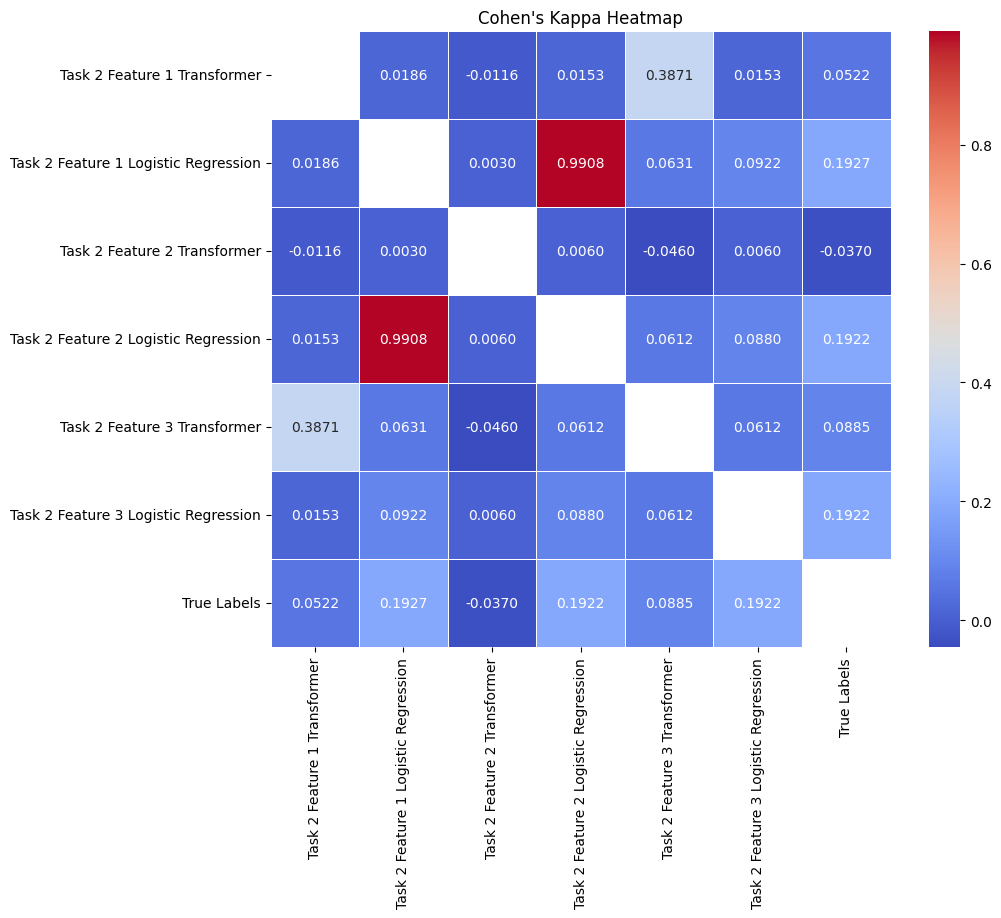
\includegraphics[]{images/CohensK.png}
  \caption{Heatmap of Cohen's Kappa Results on Multi-Class Classification Task}
  \label{fig:cohenK}
\end{figure}

The results of Cohen's K shows that for most models, the agreement between predictions are low. This is true even for the models with high accuracy. For example, the transformer models for features 1 and 2 have similar accuracies (84\% and 83.4\% respectively). However, they have a Cohen's K value of -0.0116, which, following our defined cutoff points, is no more than random chance. This indicates that on the wrong predictions, these models do not predict the same incorrect class even if they have high accuracy on correct predictions.

Between all these models, there are only 2 Cohen's K values that are greater than fair agreement. The first is between the logistic regression models of feature 1 and 2, which has a Cohen's K of 0.99, indicating an almost perfect positive agreement. This could be due to how the inputs for feature 1 and 2 are similar, and logistic regression models predict similar patterns for each of these. As such, the models predict similar classes, even for incorrect predictions.

The second is between the transformer models of feature 1 and feature 3 with a Cohen's K of 0.39, indicating substantial positive agreement. Upon inspection, predictions of the transformer models for feature 3 only predict mainly one class. This could cause a higher than expected agreement with the transformer model for feature 1, depending on how the model for feature 1 predicts incorrect predictions.

\subsubsection{Matthews Correlation Coefficient}
Each model was compared against the ground truth to calculate their MCC values. The resulting values are shown in table \ref{tab:mccTab}.

\begin{table}[h!]
  \centering
  \begin{tabular}{|p{1cm}|p{2cm}|p{2cm}|p{2cm}|p{2cm}|p{2cm}|p{2cm}|}
      \hline
      & \textbf{Task 2 Feature 1 Transformer} & \textbf{Task 2 Feature 1 Logistic Regression} & \textbf{Task 2 Feature 2 Transformer} & \textbf{Task 2 Feature 2 Logistic Regression} & \textbf{Task 2 Feature 3 Transformer} & \textbf{Task 2 Feature 3 Logistic Regression} \\
      \hline
      \textbf{MCC Score} & 0.066509038 & 0.194445905 & -0.043092423 & 0.19418937 & 0.103772985 & 0.124725893 \\
      \hline
  \end{tabular}
  \caption{MCC Scores for Each Model, Compared Against Ground Truth}
  \label{tab:mccTab}
\end{table}

The results of the MCC indicate that most models are not able to correctly predict across all classes evenly, even for models that have high accuracy. For example, the transformer models for features 1 and 2 have an accuracy of 84\%. However, they have MCC scores that indicate very poor predictions when considering performance across all classes. This could suggest that the model performs significantly worse when considering a class-to-class basis.

However, for some models that do not have high accuracy, they appear to have higher MCC scores. For example, the logistic regression models have an MCC score of about 0.12-0.19, and even the model that predicts only one class(transformer for feature 3), has an MCC score of 0.10. This particular transformer model predicted only the majority class, allowing it to minimize false positives and false negatives. As such, although they do not have a good accuracy, they are able to minimize misclassifications, leading to a decent MCC score.

%==============================
\section{Discussion}\label{discussion and conclusion}
%==============================
This report has performed the statistical tests suggested by Rainio, Tauho, and Klén\cite{statsBased} on two natural language processing tasks, namely a multi-label binary annotation task and a multi-class drug classification task. For each task, different statistical tests were applied to investigate model behaviour. 

\subsection{Multi-Label Classification Task}
Interpretation of the statistical tests on the multi-label task can be considered in three stages. First, the traditional machine learning metrics show that transformer models are able to outperform their logistic regression baselines consistently. Furthermore, the difference in features affect logistic regression and transformer models differently, albeit only slightly. Secondly, the HL values provide further support that transformers are able to outperform logistic regression models, even when considering individual label predictions. However, the HL shows that logistic regression models perform better on a label-by-label basis than suggested by their accuracy, as HL relaxes the requirement that all the labels are correctly predicted for an instance to be considered correct. Finally, Friedman's test shows that the difference in model predictions are statistically significant.


\subsection{Multi-Class Classification Task}

Interpretation of the multi-class classification task shows opposite performance when comparing traditional machine learning metrics to statistical tests. Traditional machine learning metrics show that for features 1 and 2, the transformer outperforms their logistic regression baselines. However, for feature 3, the transformer performed worse than their baseline. This behaviour highlights the difference in expected behaviours. Logistic regression learns patterns, while transformers capture language understanding, and depending on the input, learning simpler patterns could lead to better performance. 

Investigation on Cohen's K also further supports how logistic regression models learn similar patterns given similar inputs, while transformers might learn different weights with similar inputs. This leads to different incorrect predictions. Furthermore, Cohen's K can also provide insights into what incorrect predictions are done. For example, the transformer models of feature 1 and 3 have a substantial positive agreement, indicating that feature 1 might default to the majority class for incorrect predictions. While this report does not investigate this behaviour in depth, the results of Cohen's K provides an indicator of possible model behaviour that could be investigated further.

Finally, the results of the MCC scores show that transformer models do not tend to each class equally, which could support the behaviour of the transformer for feature 1 to default to a majority class. Similar low MCC scores could also indicate similar behaviour. While investigating the exact causes of these MCC scores are out of the scope of this report, MCC scores can provide indications on what the model struggles with, such as evenly predicting every class.

\subsection{Friedman's Test on Multi-Class Classification}

The application of Friedman's test on multi-class classification poses a challenge due to the output, which comes in the form of text. Friedman's test calculates differences between a series of predictions. In multi-label classification, this difference is calculated as either 1 or 0 (with 1 meaning that there is a difference between predictions and 0 as having the same predictions). However, text data such as drug names need to be preprocessed into numerical variables. While some studies have used Friedman's test on textual data by converting it into a ranking task\cite{article1}, there is no consensus on how to handle this change in features. Some methods that could be investigated could involve converting text into a word embedding such as TF-IDF, calculating the vector differences to identify distances between predictions. However, this is out of the scope of this report, but future work could be done to tackle this issue.

\section{Conclusion and Future Directions}

In conclusion, this report has shown how statistical tests, combined with traditional machine learning metrics can help to better understand model behaviour. However, it should be noted that each metric performs different functions. While statistical tests indicate model behaviour, traditional machine learning models are still important when considering practicality. For example, for multi-class classification, while the transformer models for feature 1 and 2 do not perform evenly on all classes, their accuracy would still make a transformer model preferred in performing predictions. 

In addition, while statistical tests suggest possible undesireable model behaviour, these metrics could still be misleading, such as how predicting a majority class inflates the MCC score. While some studies have suggested how MCC has advantages over F1-scores and accuracy\cite{articlesss}, these metrics should still be understood as providing ideas on model behaviour, instead of replacing traditional machine learning metrics.

Future work can investigate more sophisticated workflows to understand model behaviour based on statistical tests. In addition, the difficulty in using some statistical tests on textual data such as Friedman's test described above could be further investigated. Additional statistical tests could also be integrated, such as testing assumptions of independence, which could guide what statistical tests fit a specific task and to identify possible problems with a provided dataset\cite{article2}.

% future work could include additional statistical tests on features (e.g., chi squared tests of feature indpendence) Efficient and inefficient obviously have some feature dependence, but these are labels. nevertheless, these could be investigated

%a challenge is that NLP tasks generally uses one singular text as the input (e.g.,just the review text). However, we still show how investigating feature engineering on the text could provide deeper insights on how the model performs and increases interpretability.

% could expand into studying the use of this on different datasets because it would provide more statistical power (that the models can generalize outside of datasets)
%==============================
\newpage
\bibliographystyle{vancouver}
\bibliography{literature}
%==============================

\section{Appendix}

\subsection{Appendix A - Equations for Statistical Tests}


\textbf{Cohen's K:}

\begin{equation}
  \kappa = \frac{p_o - p_e}{1 - p_e}
  \end{equation}
  
  where:
  \begin{align*}
  p_o & = \text{relative observed agreement among raters} \\
  p_e & = \text{hypothetical probability of chance agreement}
  \end{align*}
  
  ($p_o$) is calculated as:
  
  \begin{equation}
  p_o = \frac{a + d}{a + b + c + d}
  \end{equation}
  
  ($p_e$) is calculated as:
  
  \begin{align}
    p_e &= \left(\frac{(a + b)}{a + b + c + d} \cdot \frac{(a + c)}{a + b + c + d}\right) \notag \\
    &\quad + \left(\frac{(c + d)}{a + b + c + d} \cdot \frac{(b + d)}{a + b + c + d}\right)
    \end{align}

  where:
  \begin{itemize}
      \item $a$ = Number of times both annotators agreed the sample was positive
      \item $d$ = Number of times both annotators agreed the sample was negative
      \item $b$ = Number of times Annotator A said positive but Annotator B said negative
      \item $c$ = Number of times Annotator A said negative but Annotator B said positive
  \end{itemize}

  \textbf{Matthews Correlation Coefficient:}
  \begin{equation}
    \text{MCC} = \frac{TP \cdot TN - FP \cdot FN}{\sqrt{(TP + FP)(TP + FN)(TN + FP)(TN + FN)}}
    \end{equation}

  \begin{flalign*}
    \text{where:} \\
    TP & : \text{True Positive} \\
    FP & : \text{False Positive} \\
    TN & : \text{True Negative} \\
    FN & : \text{False Negative} \\
  \end{flalign*}


\textbf{Hamming Loss:}

\[
\text{HL} = \frac{1}{N \times L} \sum_{l=1}^L \sum_{i=1}^N (Y_{i,l} \neq X_{i,l})
\]

\begin{flalign*}
\text{where:} \\
N & : \text{Number of samples} \\
L & : \text{Number of labels} \\
Y_{i,l} & : \text{True label for } i\text{th sample and } \\ 
& l\text{th label} \\
hat{y}_{ij} & : \text{Predicted label for } i\text{th sample and }\\
& l\text{th label} \\
(Y_{i,l} \neq hat{y}_{ij}) & : \text {1} \text{ if } y_{ij} \neq \hat{y}_{ij} \text{ and } 0 \text{ otherwise}
\end{flalign*}


\textbf{Accuracy, Precision, Recall, and F1-Scores:}
\begin{equation}
  Accuracy = \frac{TP+TN}{TP+TN+FP+FN}
\end{equation}

\begin{equation}
  Precision = \frac{TP}{TP+FP}
\end{equation}

\begin{equation}
  Recall = \frac{TP}{TP+FN}
\end{equation}

\begin{equation}
  F1 = \frac{2*Precision*Recall}{Precision+Recall} = \frac{2*TP}{2*TP+FP+FN}
\end{equation}

\begin{flalign*}
  \text{where:} \\
  TP & : \text{True Positive} \\
  FP & : \text{False Positive} \\
  TN & : \text{True Negative} \\
  FN & : \text{False Negative} \\
\end{flalign*}

\textbf{Friedman's Test:}

\begin{equation}
  T = \frac{12 \sum S_{ij}^2}{jk(j+1)} - 3k(j+1)
\end{equation}

where:
\begin{align*}
T & = \text{test statistic} \\
\sum S_{ij}^2 & = \text{sum of the squared sums of ranks for each prediction set} \\
j & = \text{number of prediction sets} \\
k & = \text{number of instances}
\end{align*}
\newpage
\subsection{Appendix B - Transformer Model Performances}

\begin{figure}[H]
  \centering
  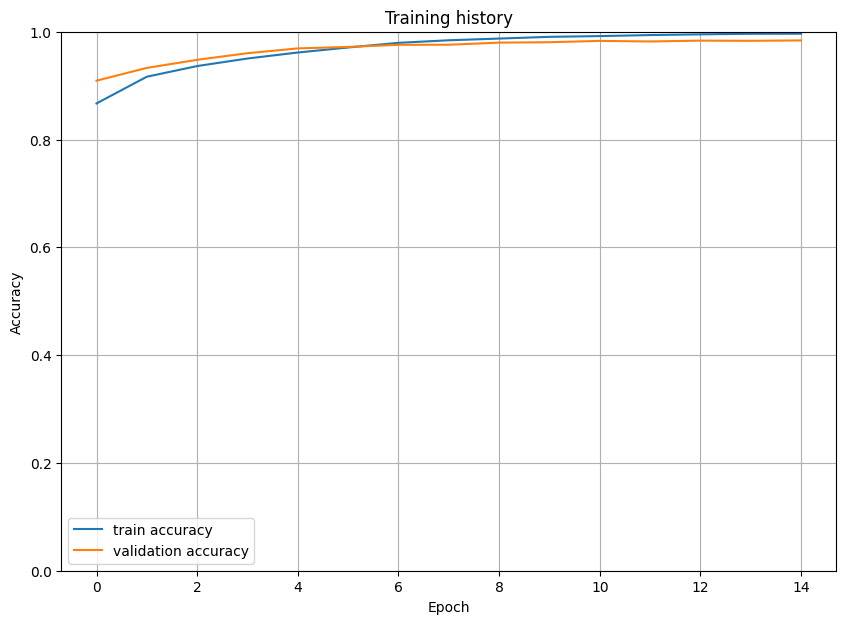
\includegraphics[]{images/model2_task1_feature1_plot.png}
  \caption{Task 1 Feature 1 Model Training (Total Training Time: 2056.51 Seconds)}
  \label{fig:t1f1plot}
\end{figure}

\begin{figure}[H]
  \centering
  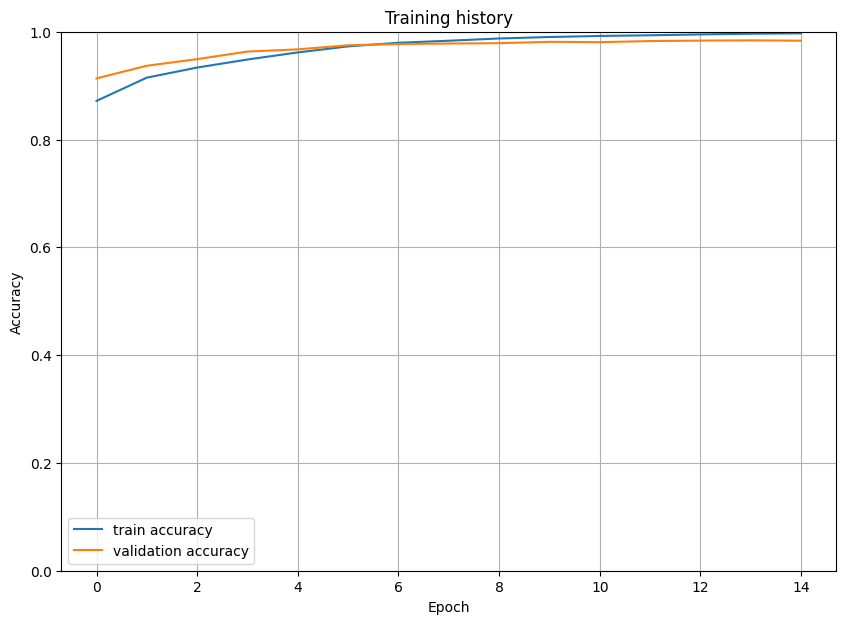
\includegraphics[]{images/model2_task1_feature2_plot.png}
  \caption{Task 1 Feature 2 Model Training (Total Training Time: 2037.76 Seconds)}
  \label{fig:t1f2plot}
\end{figure}

\begin{figure}[H]
  \centering
  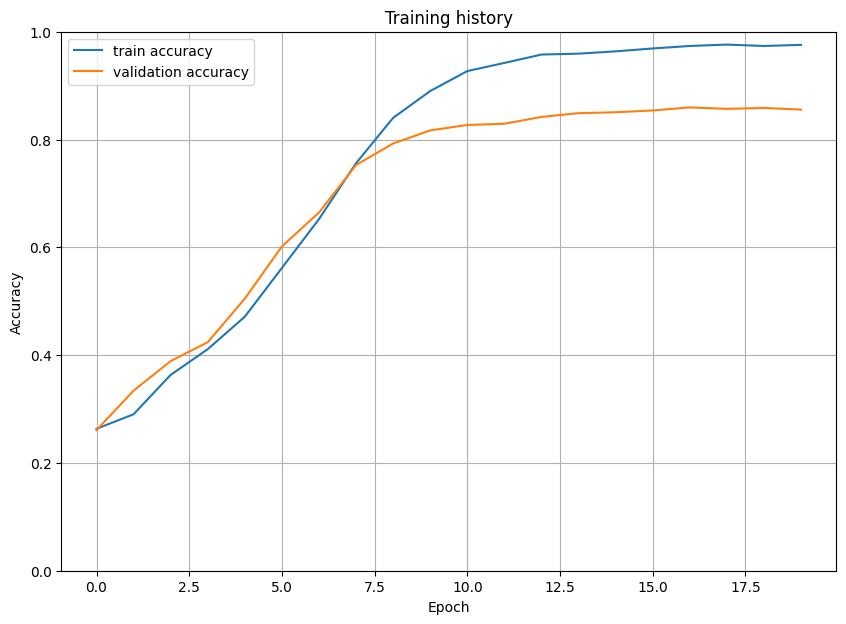
\includegraphics[]{images/model2_task2_feature1_plot.png}
  \caption{Task 2 Feature 1 Model Training (Total Training Time: 7471.89 Seconds)}
  \label{fig:t2f1plot}
\end{figure}

\begin{figure}[H]
  \centering
  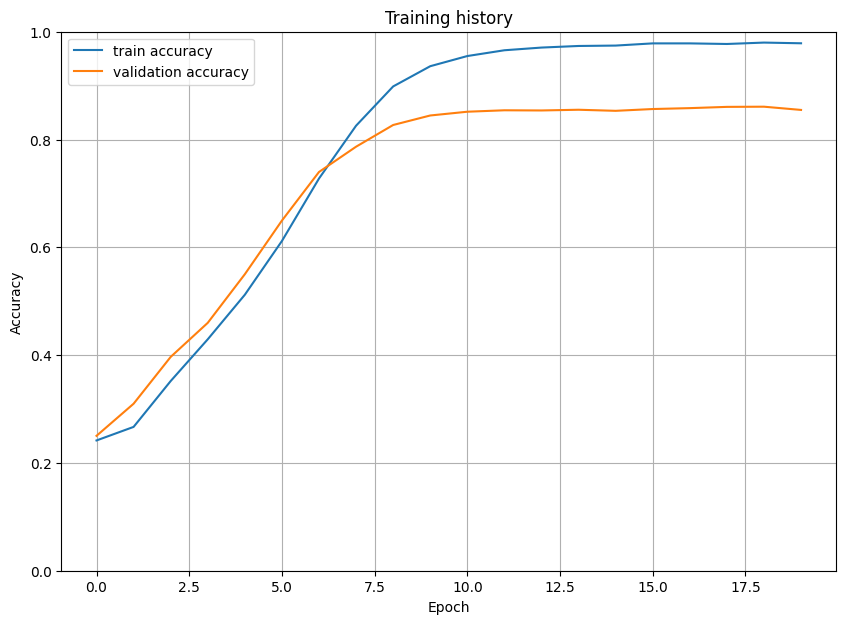
\includegraphics[]{images/model2_task2_feature2_plot.png}
  \caption{Task 2 Feature 2 Model Training (Total Training Time: 6587.32 Seconds)}
  \label{fig:t2f2plot}
\end{figure}

\begin{figure}[H]
  \centering
  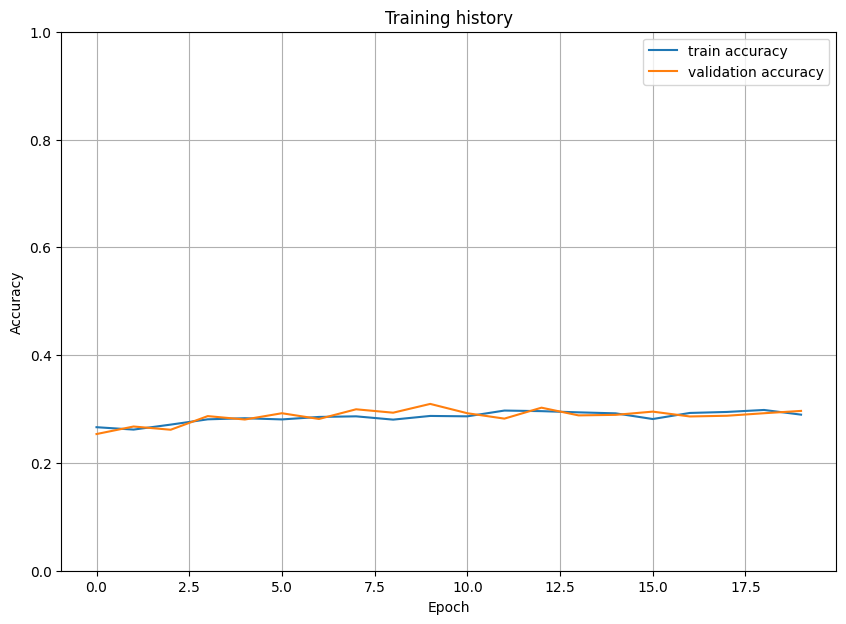
\includegraphics[]{images/model2_task2_feature3_plot.png}
  \caption{Task 2 Feature 3 Model Training (Total Training Time: 6590.17 Seconds)}
  \label{fig:t2f3plot}
\end{figure}
\newpage
\subsection{Appendix C - Source Code}

%\includepdf[page=-]{pdf_final_code.pdf}
%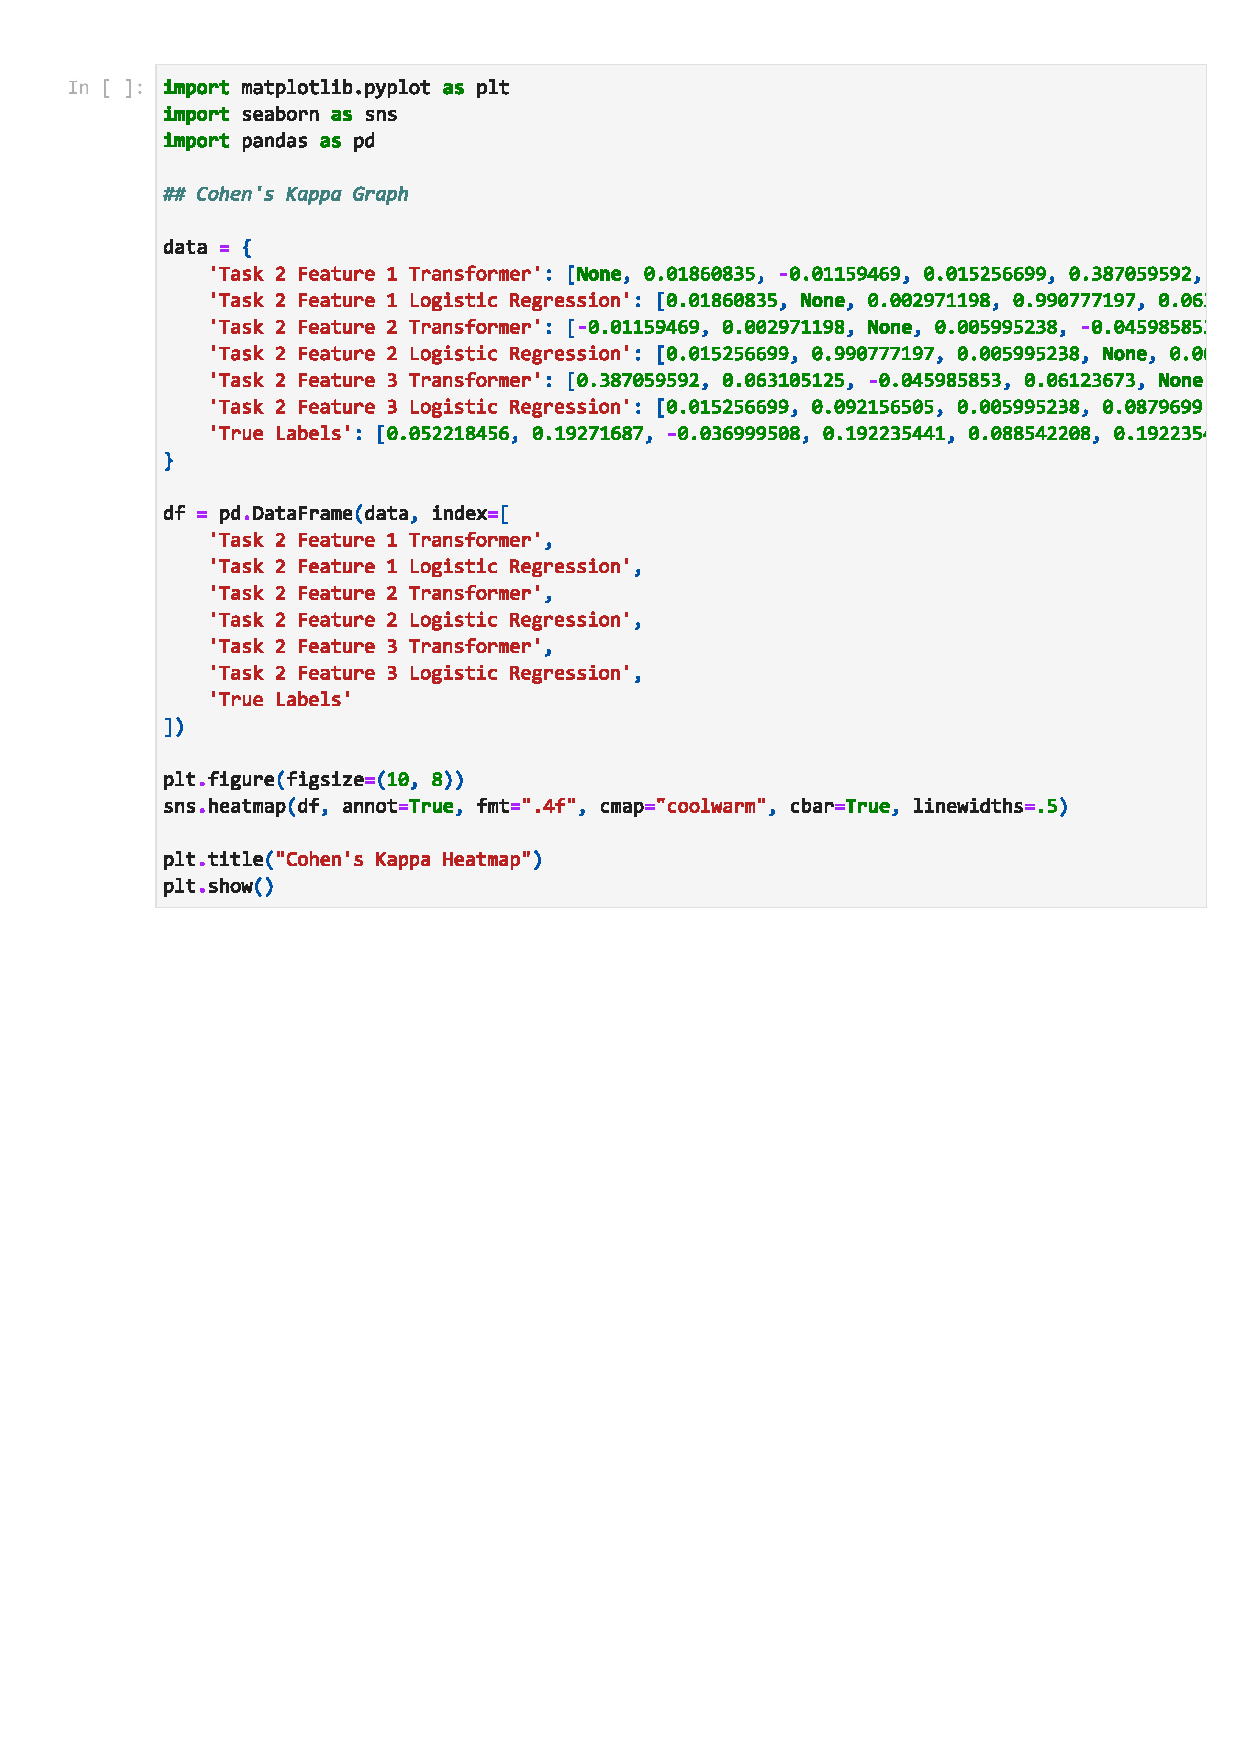
\includepdf[page=-]{pdf_final_visualization_code.pdf}
\end{document}
